\documentclass[11pt]{article}
\usepackage{graphicx}
\usepackage{fullpage}
\usepackage{amsfonts}
\usepackage{amssymb}
\usepackage{amsmath}
\usepackage{xcolor}
\usepackage{algorithm}
\usepackage{algorithmic}
\usepackage{enumitem}
\usepackage{fourier}
\usepackage[normalem]{ulem}


\newcommand{\F}{\mathbb{F}}
\newcommand{\np}{\mathop{\rm NP}}
%\newcommand{\binom}[2]{{#1 \choose #2}}

\newcommand{\mnote}[1]{{\color{red} [Madhu: #1]}}
\newcommand{\achnote}[1]{{\color{orange} [Sitan: #1]}}

\newcommand{\Z}{{\mathbb Z}}
\newcommand{\vol}{\mathop{\rm Vol}}
\newcommand{\conp}{\mathop{\rm co-NP}}
\newcommand{\atisp}{\mathop{\rm ATISP}}
\renewcommand{\vec}[1]{{\mathbf #1}}
\newcommand{\cupdot}{\mathbin{\mathaccent\cdot\cup}}
\newcommand{\mmod}[1]{\ (\mathrm{mod}\ #1)}
\newcommand{\code}[1]{$\texttt{#1}$}


\setlength{\parskip}{\medskipamount}
\setlength{\parindent}{0in}

\begin{document}

%{\color{brown} Changes after test solvers started looking indicated in brown.}

%{\color{red} Changes after release indicated in red.}

        \section*{CS 124 Homework 3: Spring 2024}

%{\color{brown}        \sout{\textbf{Your name:}}}

        \textbf{Collaborators: }

        \textbf{No. of late days used on previous psets: }\\
        \textbf{No. of late days used after including this pset: }

Homework is due {\color{blue} Wednesday Feb 28 at 11:59pm ET}. 
{\color{purple} Please remember to select pages when you submit on gradescope. Each problem with incorrectly selected pages will lose 5 points.}

Try to make your answers as clear and concise as possible;
style may count in your grades. Assignments must be submitted in pdf format on Gradescope. If you do assignments by hand, you will need to scan your papers to turn them in.


{\bf Collaboration Policy:} You may collaborate on this (and all problem sets) only with other students currently enrolled in the class, and of course you may talk to the Teaching Staff or use Ed. You may also consult the recommended books for the course and course notes linked from the timetable. You may not use generative AI or large language models, or search the web for solutions, or post the questions on chat forums. Furthermore, you must follow the "one-hour rule" on collaboration.  You may not write anything that you will submit within one hour of collaborating with other students or using notes from such sources. That is, whatever you submit must first have been in your head alone, or notes produced by you alone, for an hour. Subject to that, you can collaborate with other students, e.g. in brainstorming and thinking through approaches to problem-solving.


For all homework problems where you are asked to give an algorithm, you must prove the correctness
of your algorithm and establish the best upper bound that you can give for the running time. Generally
better running times will get better credit; generally exponential-time algorithms (unless specifically asked
for) will receive no or little credit. You should always write a clear informal description of your algorithm
in English. You may also write pseudocode if you feel your informal explanation requires more precision
and detail, but keep in mind pseudocode does NOT substitute for an explanation. Answers that consist
solely of pseudocode will receive little or no credit. Again, try to make your answers clear and concise.



\section*{Problems}
\begin{enumerate}

\item {\bf Detecting whether an edge lies in an MST (10 points)}

\begin{enumerate}
    \item {\bf (5 points)} Let $G$ be a weighted graph in which all edge weights are distinct. Prove that an edge $e$ of a graph $G$ belongs in some MST of $G$ if and only if the following property holds: for every cycle in $G$ that contains $e$, the edge with the highest weight is not $e$.
    \begin{quote}
      \color{purple}
      \textbf{Direction 1}: If $e$ belongs in some MST of $G$, then for every cycle of $G$ containing $e$, the edge wigh the highest weight is not $e$. 

      \medskip
      Let $M$ be any MST of $G$ containing $e$. Let $c$ be any edge in $G$ but not $M$ such that adding $c$ to $M$ produces a cycle containing $e$. By definition of cycle, the vertices connected by $e$ now have a path to each other not using $e$. So, remove $e$ from $M$. Because $e$ is no longer in the cycle, the cycle is broken. This leaves a new spanning tree in the graph. This new spanning tree is identical to the previous spanning tree except it contains $c$ instead of $e$. Because edge weights are distinct, this new spanning tree with $c$ is either lighter or heavier than the tree using $e$. If it were lighter, then that would contradict the assumption that $M$ is an MST using $e$ because it would have used $c$ instead. So, it must be heavier. This implies that $c$ is heavier than $e$ and thus $e$ is not the heaviest edge. This proves the assertion that for every cycle of $G$ containing $e$, the edge with the highest weight is not $e$.

      \medskip
      \textbf{Direction 2}: If for every cycle in $G$ containing $e$ the edge with the highest weight is not $e$, then $e$ belongs in some MST of $G$. 

      \medskip
      Let $C$ be any cycle in $G$ containing $e$. Let $h$ be the heaviest edge in that cycle. By the claim's assumption, assert that $e$ and $h$ are distinct. Consider any partitioning of the vertices in $C$ such that the only two edges in $C$ crossing the cut are $e$ and $h$. By the cut property, the least of these edges will be in an MST of $G$. Because $e$ is lighter than $h$, the construction of such an MST will choose $e$ over $h$ to connect the two cuts, implying that $e$ will be in some MST of $G$.
    \end{quote}
    \item {\bf (5 points)} Given an edge $e$ in $G$, give an algorithm that outputs YES if there exists an MST of $G$ that contains $e$, and NO otherwise. Your algorithm must have runtime asymptotically faster than the algorithms given in class for finding MSTs. You must describe your algorithm, prove its correctness and state its run time. You need not prove the runtime. (You may use the result from Part (a) even if you did not prove it.)
      \begin{quote}
        \color{purple}
        Consider this algorithm. In the algorithm, let $v_1$ and $v_2$ denote the two vertices connected by $e$:
        \begin{enumerate}
          \item Remove $e$ from $G$. 
          \item Initialize a Visited set and a PathWeights set for use in the DFS.
          \item Run a modified DFS on the graph starting at $v_1$. In the DFS, track the maximum-weight edge traversed on the current path. If the DFS ever reaches $v_2$, add the maximum weight of that path to the PathWeights set. 
          \item Let $G'$ be the $G$ without $v_2$. If DFS did not visit every vertex in $G'$, return NO.
          \item If the PathWeights set is empty, return YES. 
          \item If $e$ is heavier than any value in PathWeights, return NO. Else, return YES.
        \end{enumerate}

        \textbf{Correctness}: \\ 
        \textit{If the algorithm returns something, it is correct about the MST membership of e}:  First, if the DFS didn't visit every vertex in $G'$, then the graph is not connected even with $e$ added back. The vertex $v_2$ is excluded because it might be unreachable without $e$. If the graph is not connected, then a spanning tree cannot exist, and $e$ can subsequently not be part of such a tree. Here, it's correct to return NO. Otherwise, the DFS will have collected the maximum weight edges on every path from $v_1$ to $v_2$. If no such path exists, then $e$ is the only edge the connect $v_1$ and $v_2$. For the tree to span, it must include $e$. So, it's correct to return YES. Finally, if $e$ is lighter than the heaviest edge on every path from $v_1$ to $v_2$, then $e$ is also not the heaviest edge in every cycle containing $e$. By part $a$, it is correct to return YES. Otherwise, NO is returned, which is also correct due to the iff nature of part $a$. 

        \medskip
        \textit{If e is in an MST of G, then the algorithm returns YES}: If $e$ is in an MST of G, then such an MST exists. This implies all vertices in the graph are connected, and the DFS will visit the entire graph except possibly $v_2$. So, the algorithm will not return NO from that case. If $e$ is the only edge to $v_2$ from the rest of the graph, then the algorithm will correctly return YES because $e$ is required to make the tree span the entire graph. Otherwise, according to part $a$, because $e$ is in an MST of G, the maximum-weight edges collected in the PathWeights set must all be greater than $e$. The final check will observe this and return YES. 

        \textbf{Runtime}: \\
        The visited set is already part of DFS. Tracking the maximum weight edge along a path and maintaining PathWeights takes $O(1)$ time. So, DFS still takes time $O(E + V)$ where $E$ is the number of edges and $V$ is the number of vertices. This also bounds the size of PathWeights. Thus, the runtime is that of the DFS, $O(V + E)$. 
      \end{quote}
\end{enumerate}

\item {\bf Maximal independent set in an evolving graph (30 points):}

%{\color{blue} [sitan: experimental question to test student on understanding of amortized analysis]}

Given an undirected graph $G = (V,E)$, we say that a subset $S\subset V$ is an \emph{independent set} if no two vertices in $S$ are connected by an edge. We say that $S$ is a \emph{maximal independent set (MIS)} if $S$ is an independent set and furthermore there is no strict superset $T$ (i.e., a set $T$ with $S \subsetneq T$) which is also an independent set. In this problem we will explore the running time of algorithms computing and maintaining maximal independent sets in graphs with $n$ vertices, $m$ edges and with maximum degree $\Delta$ (i.e., every vertex $u \in V$ has at most $\Delta$ edges touching it.) 



\begin{enumerate}
    \item {\bf (5 points)} Give an algorithm that finds a maximal independent set of $G$, given $G$ in the adjancency list representation. (You must describe your algorithm fully and give a brief explanation of why it is correct. You should state your runtime but you don't need to prove it.) 
    \begin{quote}
      \color{purple}
      Consider this algorithm: Given an adjacency list graph called $\texttt{adj}$, initialize an empty set called $\texttt{ind\_set}$. While $\texttt{adj}$ is not empty, pop a vertex $\texttt{v}$ and its edges from $\texttt{adj}$ and add $\texttt{v}$ to $\texttt{ind\_set}$. Then, for every neighbor in edges, delete that neighbor from $\texttt{adj}$. At the end, return $\texttt{ind\_set}$. Here's pseudocode for such an algorithm:
      \begin{verbatim}
fn max_ind_set(adj: adjacency list graph) -> Set(vertices):
  let ind_set = {};
  while adj is not empty:
      let (v, edges) = pop entry from adj;
      ind_set.add(v);
      for neighbor in edges:
          adj.delete(neighbor);
  return ind_set;
      \end{verbatim}
      
      \textbf{Correctness}: \\ 
      \textit{Lemma}, $\texttt{ind\_set}$ is an independent set and the vertices in $\texttt{adj}$ share no edges with vertices in $\texttt{ind\_set}$. 
      \begin{itemize}
        \item Base case: $\texttt{ind\_set}$ is an independent set initially because it's empty. There are also trivially no edges between $\texttt{ind\_set}$ and $\texttt{adj}$.
        \item Inductive hypothesis: after $0 \leq n$ iterations of the \texttt{while} loop, (1) $\texttt{ind\_set}$ is an independent set and (2) vertices \texttt{adj} share no edges with vertices in $\texttt{ind\_set}$. 
        \item Inductive step: at the $n + 1$ iteration of the while loop, $\texttt{v}$ is popped from $\texttt{adj}$. By the inductive hypothesis, $\texttt{v}$ shares no edges with vertices in $\texttt{ind\_set}$. So, adding it to $\texttt{ind\_set}$ maintains $\texttt{ind\_set}$ as an independent set. Then, every vertex sharing an undirected edge with $\texttt{v}$ is deleted from $\texttt{adj}$. After this, $\texttt{adj}$ contains no vertices with edges to $\texttt{v}$. By the inductive hypothesis, it also contains no edges with vertices previously in $\texttt{ind\_set}$. This preserves the inductive hypothesis and thus proves the claim inductively.
      \end{itemize}

      \medskip
      \textit{Proof of correctness}: From the lemma above, assert that once $\texttt{adj}$ is empty, $\texttt{ind\_set}$ is an independent set and there are no vertices remaining in the graph that don't share an edge with a vertex in $\texttt{ind\_set}$. This implies that the value returned from $\texttt{max\_ind\_set}$ is a maximal independent set. Similarly, because a maximal independent set will always exist in a non-empty graph, if a maximal independent set exists in the input graph, one is found and returned by $\texttt{max\_ind\_set}$. 

    \medskip
    \textbf{Runtime}: \\ 
    The algorithm iterates every vertex and every edge in the graph, so it runs in time $O(V + E)$. That assumes the input adjacency list is encoded as a HashMap with key vertex and value HashSet of neighbor vertices. I further assume insertion and deletion on those data structures take an average of $O(1)$ time.
    \end{quote}
\end{enumerate}

Now suppose the graph $G$ is changing over time, and we want to maintain a maximal independent set of this graph without having to recompute it from scratch every time $G$ is updated. Concretely, suppose that in each time step, some edge is either added to or deleted from $G$. Our basic data structure simply maintains a set $S \subseteq V$ in the form of an array indexed by $V$ such that $S[u]=1$ if $u \in S$ and $0$ otherwise.

\begin{enumerate}[resume]
    \item {\bf (0 points, not to be turned in)} Prove that the adjacency lists can be maintained with $O(\Delta)$ cost per insertion and deletion. (You may assume you have a solution to this problem in future parts even if you did not solve it.)
    \item {\bf (7 points)} Describe algorithms INSERT$(e)$ and DELETE$(e)$ to maintain $S$ under edge insertions and deletions respectively. Give upper bounds on the runtime of both operations. \label{part:2c} (Your algorithm and its claimed run times must be correct, but you need not prove these. Note that for full credit your runtimes should depend only on $\Delta$ and not on $n$.)
    \begin{quote}
      \color{purple}
      Note: While it's not stated in the prompt, I'm assuming my methods have read access to the graph. 

      \medskip 
      Consider these three functions:
      \begin{itemize}
        \item \code{add\_if\_able}: Accepts a vertex \code{v}. If no neighbors of \code{v} are in \code{S}, then add \code{v} to \code{S}.
        \item \code{insert}: Accepts an edge between vertices \code{v1} and \code{v2}. If both of the vertices are in \code{S}, then remove \code{v1} from \code{S} and call \code{add\_if\_able} on all of neighbors of \code{v1}.
        \item \code{delete}: Accepts an edge between vertices \code{v1} and \code{v2}. If exactly one of the edge endpoints is in \code{S}, call \code{add\_if\_able} on the vertex not in \code{S}.
      \end{itemize}
      Here's pseudocode for these algorithms:
      \newpage
\begin{verbatim}
DynamicMaximalIndSet {
    Independent set tracker S;

    fn add_if_able(v: Vertex, graph: &Graph):
        for neighbor in graph[v]:
            if S[neighbor] == 1:
                return
        S[v] = 1;

    fn insert((v1, v2): edge, graph: &Graph):
        if S[v1] != 1 or S[v2] != 1:
            return;
        S[v1] = 0;
        for neighbor in graph[v1]:
            add_if_able(neighbor, graph);

    fn delete((v1, v2): edge, graph: &Graph):
        if S[v1] == 0 and S[v2] == 0:
            return;
        Assert S[v1] and S[v2] are not both 1;
        let v = the side of the edge not in S;
        add_if_able(v, graph);
}
\end{verbatim}
    While proofs are not required, here's my reasoning for each along with runtime:
    \begin{itemize}
      \item \code{add\_if\_able}: If a vertex has no edges to vertices in the independent set, then it can be added to the independent set. This iterates the edges of a vertex. If each vertex has $O(\Delta)$ edges, then this takes $O(\Delta)$ time.
      \item \code{insert}: If the new edge is between two vertices not in \code{S}, both of those vertices must already have some neighbor in S preventing them from joining S. This requires no updates. Similarly, if one of the vertices is in \code{S}, then the other edge has yet another reason it cannot be in \code{S}. That case should also be igored. If both vertices are already in \code{S}, then one of them must be removed to maintain the independent set property. I arbitrarily chose \code{v1}. Removing \code{v1} might enable any of its neighbors to now join \code{S}, so they must be considered. However, either they cannot join because of a different neighbor in \code{S}, or they can join, giving all their neighbors yet another neighbor in \code{S}. Because of that, only one degree of separation from the initially-removed vertex must be considered. Considering all the neighbors of all the neighbors of the removed vertex takes time $O(\Delta^2)$.
      \item \code{delete}: If an edge is deleted between two vertices not in \code{S}, then both vertices still must have some neighbor in \code{S} preventing them from joining \code{S}. This implies no change. Simiarly, it should be impossible to delete an edge between two vertices in \code{S} because of the independent set property. Finally, if only one of the vertices is in \code{S}, the vertex not in \code{S} might now be able to join \code{S}. Checking this gives the function a total runtime of $O(\Delta)$.
    \end{itemize}
    \end{quote}
    \item {\bf (3 points)} For every integer $\Delta>0$  describe an example (i.e., a graph, an MIS, and an edge to be inserted) such that the number of queries to $S$ for inserting an edge asymptotically match your upper bound from Part~\ref{part:2c}. 
      \begin{quote}
        \color{purple}
        Let $G$ be a complete graph with $n$ vertices. By definition, every vertex has $n - 1$ edges, so $\Delta$ is $n - 1$. Because it's a complete graph, only one vertex $v_0$ will initially be in $S$. Choose another vertex $v_k$ in the graph and remove its edge with $v_0$. Because $v_0$ was the only vertex in $S$, $v_k$ will now also be added to $S$. Now, re-insert that edge. Doing so will cause $v_0$ to be removed from the graph. Then, for each of $v_0$'s neighbors $v_{nb}$, each of the $v_{nb}$'s neighbors will be inspected to see if $v_{nb}$ can be added to the graph. Because the graph is complete, this will result in $(n - 1) * (n - 1)$ loop iterations, which will have $\Theta(\Delta^2)$ runtime. Allowing any $n > 1$ will demonstrate this behavior for any integer $\Delta > 0$. 
      \end{quote}
\end{enumerate}

To speed up the runtimes from Part~\ref{part:2c}, suppose we decide to additionally maintain 
an array $A$ indexed by $V$, such that for every $u\in V$, $A[u]$ counts the number of neighbors of $u$ that are in $S$. (So $A[u] = |\{v \in V | v \in S, (u,v) \in E\}|$.) 

\begin{enumerate}[resume]
    \item {\bf (5 points)} Give algorithms A-INSERT and A-DELETE that maintains both $S$ and $A$ under edge insertions and deletions. (While any correct polynomial-time algorithm will get you full points, needlessly inefficient algorithms will lose points in the next part!)
    \begin{quote}
      \color{purple}
      Consider this set of algorithms: 
      \begin{itemize}
        \item \code{add\_if\_able}: Given a vertex \code{v}, if \code{A[v]} is greater than zero, return. Else, add \code{v} to \code{S} and, for each \code{neighbor} of \code{v}, increment \code{A[neighbor]} by one.
        \item \code{insert}: Given an edge between \code{v1} and \code{v2}, if neither vertex is in \code{S}, return. If exactly one of the vertices \code{v} is in \code{S}, then increment \code{A[v]} by one and return. Else, remove \code{v1} from \code{S}, set \code{A[v1]} to one, and, for each neighbor of \code{v1} except \code{v2}, decrement \code{A[neighbor]} by one and call \code{add\_if\_able} on that \code{neighbor}.
        \item \code{delete}: Given an edge between \code{v1} and \code{v2}, if neither edge is in \code{S}, return. Assert that the vertices are not both in \code{S}. Let \code{v} be the side of the deleted edge not in \code{S}. Decrement \code{A[v]} by one and call \code{add\_if\_able} on \code{v}.
      \end{itemize}
      Pseudocode for this algorithm: 
      \newpage
    \begin{verbatim}
ADynamicMaximalIndSet {
    Independent set tracker S;
    Neighbor count tracker A;

    fn add_if_able(v: Vertex, graph: &Graph):
        if A[v] > 0:
            return;
        S[v] = 1;
        for neighbor in graph[v]:
            A[neighbor] += 1;

    fn insert((v1, v2): edge, graph: &Graph):
        if S[v1] == 0 and S[v2] == 0:
            return;
        if S[v1] == 0 or S[v2] == 0:
            let v = the side of the edge not in S;
            A[v] += 1;
            return;

        S[v1] = 0;
        A[v1] = 1;
        for neighbor in graph[v1] excluding v2:
            A[neighbor] -= 1;
            add_if_able(neighbor, graph);

    fn delete((v1, v2): edge, graph: &Graph):
        if S[v1] == 0 and S[v2] == 0:
            return;
        Assert S[v1] and S[v2] are not both 1;
        let v = the side of the edge not in S;
        A[v] -= 1;
        add_if_able(v, graph);
}
    \end{verbatim}

    Justification for each method: 
    \begin{itemize}
      \item \code{add\_if\_able}: If \code{v} has any neighbors in \code{S}, then it does not belong in \code{S} by definition of independent set. Otherwise, it should be added. After it's added, all of its neighbors' \code{A} counts must be updated to reflect that \code{v} is now in \code{S}.
      \item \code{insert}: If neither \code{v1} nor \code{v2} is in \code{S}, then no trackers need to be updated. If exactly one vertex in the edge is in \code{S}, then the side not in \code{S} should be updated to reflect its additional edge with a vertex in \code{S}. Otherwise, if both vertices are in \code{S}, then arbitrarily choose \code{v1} to be dropped. Doing so implies that \code{v1} now has one edge into \code{S} with \code{v2} and no others because it was previously in the independent set. Each non-\code{v2} neighbor of \code{v1} just lost an edge into \code{S} and should be decremented and reconsidered for membership in \code{S}. 
      \item \code{delete}: This is almost identical to before except the vertex not in \code{S} now has its count into \code{S} decremented due to the edge deletion.
    \end{itemize}
      
    \end{quote}
    \item {\bf (10 points)} Assume that initially the graph $G$ is empty (no edges), and $S$ consists of all vertices in $V$. Give an amortized analysis proof that after $T$ updates to $G$, the total runtime of the operations is at most $O(\Delta\cdot T)$. (Hint: Consider a charging scheme that charges the runtime of adding a vertex to $S$ to the vertex itself. You should be careful to pay this charge when the same vertex is deleted from $S$!)
      \begin{quote}
        \color{purple}
        Let there be two types of events:
        \begin{itemize}
          \item Type 1: A vertex is added to S. 
          \item Type 2: A vertex is removed from S. 
        \end{itemize}
        Consider an amortization scheme where the cost of a Type 1 action is completely paid by a Type 2 action on the same vertex. Analyze each method in the data structure for its complexity:
        \begin{itemize}
          \item \code{add\_if\_able}: The first case is $O(1)$. Otherwise, in the worst case, this function runs in $O(\Delta)$ to update every neighbor of a vertex added to $S$. Because this only happens during a Type 1 event, defer all of this $O(\Delta)$ cost to the Type 2 action removing the same vertex from $S$. Doing so allows \code{add\_if\_able} to run in charged $O(1)$ time. 
          \item \code{insert}: The first two cases are $O(1)$. Otherwise, if both vertices are in \code{S}, then \code{v1} must be removed from \code{S}. The Type 2 update itself is $O(1)$, but it also incurs the deferred Type 1 cost of $O(\Delta)$, which is now paid off. Then, for every neighbor of \code{v1}, perform an $O(1)$ update to \code{A} and call \code{add\_if\_able}. Under the charging scheme, \code{add\_if\_able} costs a charged $O(1)$ time, and calling that on every neighbor costs $O(\Delta)$. Thus, \code{insert} costs at most $O(\Delta)$.
          \item \code{delete}: The first case is $O(1)$. Otherwise, an $O(1)$ update is made followed by \code{add\_if\_able}. By the charging argument, \code{add\_if\_able} costs $O(1)$ now, so \code{delete}'s charged cost is $O(1)$. 
        \end{itemize}

        The graph starts out with every vertex in \code{S}, so initial operations can only cause constant-time cases or vertices to be deleted from $S$. That implies paying for insertions that were never charged, which balances out later insertions that are never paid for through deletion. Otherwise, for every insertion that's eventually deleted, there's a charged cost of $O(\Delta)$ and a paid cost of $O(\Delta)$. Because the number of possible insertions and deletions bound each other, this yields a final cost across $T$ operations of $O(T \cdot \Delta)$ time.
      \end{quote}
\end{enumerate}

\iffalse{ 
We maintain a subset $S$ at every time step, and upon seeing an update in $G$, we need to update $S$ to be a maximal independent set in the new graph. It turns out that a useful data structure to keep around is an array $A$ indexed by $V$, such that for any $i\in V$, the $i$-th entry of the array $A$ is the number of $j\in S$ for which $(i,j) \in E$.

\begin{enumerate}[resume]
    \item {\bf (5 points)} Suppose some edge $(i,j)$ gets removed from $G$. How should one update $A$ and $S$? What if instead, some edge $(i,j)$ gets added to $G$?
    \item {\bf (5 points)} In either case, at most how many insertions would one have to make to $S$? At most how many deletions? At most how many of the entries of $A$ would have to be modified?
    \item {\bf (15 points)} Give an amortized analysis proof that after $N$ updates to $G$, the total number of insertions/deletions to $S$ and modifications to $A$ is bounded by $O(N\Delta)$. 
    
    (Hint: consider the ``total cost'' of deleting a vertex $v$ from $S$, both in terms of the updates to $S$ and $A$ that are needed when it has just been deleted, as well as the updates that are needed at some later point if/when it gets added back to $S$)
\end{enumerate}
}\fi 

% \item {\bf Network Construction Minimization (20 points):} 
% \newcommand{\cost}{\mathrm{cost}}

% Major shipping company Nile, headquartered in Seeyatill, henceforth $s$, wants to connect its $n$ warehouses to the source warehouse at $s$, by building a series of ``links''. Specifically, after the network is established, for every warehouse $i$ there is a path via a series of links from $s$ to $i$. Links can only be built between certain pairs $(i,j)$ of warehouses. For each such pair, there's a positive integer distance $d_{i,j}$ between them. Building a link from warehouse $i$ to warehouse $j$ requires buying $d_{i,j}$ units of construction materials for a cost of \$1 each and then shipping them from $s$ to warehouse $i$, but shipping construction materials can only be done along existing links, and shipping the complete set of construction materials for one link a distance of 1 costs \$1. That is, if there's a path $s \to i_1 \to \cdots i_t \to i$ which connects $s$ to $i$, then a link $(i,j)$ can be built for a cost of $d_{i,j} +C(i)$, where $C(i) = d_{s,i_1} + d_{i_1,i_2} + \cdots + d_{i_t,i}$. (We can only add a link $(i,j)$ if $i$ is previously connected to the source $s$. Note that the cost of building a link (i,j) depends on which of $i$ and $j$ the construction materials are sent to, but links can be built and used in both directions.)

% Your goal in this problem is to give an algorithm that outputs a sequence of links to be constructed such that they connect all the warehouses as cheaply as possible. (I.e., if your sequence is $(i_1,j_1),\ldots,(i_t,j_t)$ then you should minimize $\sum_{\ell=1}^t \cost(i_\ell,j_\ell)$.) 


\item {\bf Sorta sorting with heaps (24 points)} Explain how to solve the following two problems using heaps.
(No credit if you're not using heaps!)  
\begin{enumerate}
    \item {\bf (12 points)}
    Give an $O(n \log k)$
algorithm to merge $k$ sorted lists with $n$ total elements into one
sorted list.
\begin{quote}
  \color{purple}
  Note: My solution assumes (1) all of the $k$ input lists are non-empty and (2) the lists are linked lists with $O(1)$ cost to push and pop at the head and tail. 
  
  \medskip
  Consider this algorithm: Given a list of linked lists, first initialize pointers for the output head and tail. Create a sentinel node at the head with value $-\infty$ and point the tail to it. Also initialize a min heap for linked list nodes keyed by node value. Then, for each input linked list, push the head onto the heap. (Note: this could also use \code{heapify}, but it doesn't change asymptotic runtime). Finally, while the heap is not empty, pop a node, push its child back onto the heap if a child exists, set the popped node's child to empty, set the tail's next node to the popped node, and progress the tail pointer to the popped node that was just added. At the end, return the node after the sentinel. Pseudocode for this algorithm: 

  \begin{verbatim}
fn merge_sorted_lists(lists: List of Lists) -> List:
    let head = sentinel node(val = -inf, child = none);
    let tail = head;
    
    let heap = MinHeap of list nodes sorted by head node value;
    for list_head in lists:
        heap.push(list_head);
    
    while heap is not empty:
        let node = heap.pop();
        let child = node.next;
        if child is not empty:
            heap.push(child);
        node.next = empty list;
        tail.next = node;
        tail = tail.next;

    return head.next;
  \end{verbatim}

  \textbf{Correctness}: \\ 
  Begin by establishing the following claim: After $0 \leq m < n$ iterations of the while loop, (1) every node in the result list is less than or equal to every node in any list in the heap, (2) every node in the result list beginning at \code{head} is sorted, and (3) the length of the result list is $m + 1$. Prove by induction:
  \begin{itemize}
    \item Base case: At iteration $m = 0$, \code{head} has not been modified. The sentinel's value is $-\infty$, which is less than every node in every list in the heap. A list of length $1$ is trivially sorted, and the list has length $m + 1 = 0 + 1 = 1$. This establishes the base case.
    \item Inductive hypothesis: Assume after $0 \leq m < n$ iterations of the while loop, the claim holds. 
    \item Inductive step: At the $m + 1$ iteration of the while loop, the \texttt{next} entry is popped from the heap, made childless, and added to the result list. If it exists, the child \code{next} is added back to the heap such that only one total node is removed from the combined lists of the heap. Each input list is sorted, so the $k$ values used as keys in the heap are the least values of their lists. Because it's a min heap, the least of all these values is at the top of the heap, implying that popping it removes the least value among all nodes of all lists in the min heap. When this is popped and added to the result list, it is now less than or equal to every node remaining in any list in the heap. This proves point (1). Because the popped node was in the heap at time $m$, assert by the inductive hypothesis that it was greater than every node in the result list. Consequently, because the result list was sorted least to greatest, when the popped node is added to the end of the result list, the result list remains in sorted least to greatest order with this new greatest node at the end. This proves point (2). By the inductive hypothesis, the size of the result list at step $m$ was $m + 1$. Adding this new node yields a result list of size $(m + 1) + 1$, which proves point (3). The inductive step is thus established, and, by induction, the claim must be true. 
  \end{itemize}

  \medskip
  Applying the proof above, after the while loop has executed $n$ times, the result list will be sorted and of length $n + 1$. Removing the $-\infty$ sentinel node yields the $n$ input values still sorted least to greatest. So, if a sorted order of $n$ input values exists, the algorithm returns it.

  \medskip
  The only thing this algorithm returns is the linked list beginning after head. by the induction proof above, such a list is a length-$n$ list composed of the input elements in sorted order. So, the only thing the algorithm returns is a length-$n$ sorting of the input elements. 

  \medskip
  By these two cases, the algorithm must be correct.

  \textbf{Runtime}: \\ 
  Initializing the linked list takes $O(1)$ time. Assuming the input lists are not empty, the time to iterate all input lists is bounded by the number of nodes in all lists, $n$. Each list requires one insertion into the heap, and the heap only ever has one entry for each of the $k$ lists. So, each insertion into the heap requires time $O(\log k)$. This yields an initialization complexity of $O(n \log k)$. Using heapify under the same assumptions would take $O(n)$, but it doesn't reduce overall runtime. 

  \medskip
  Then, because one node is removed from one of the non-empty lists at each iteration of the \code{while} loop, the \code{while} loop iterates at most $n$ times. For each iteration, a heap \code{pop} and \code{push} occur. Because the heap contains at most one entry for each of the $k$ input lists, the heap never exceeds size $k$. This gives \code{push} and \code{pop} a cost of $O(\log k)$ time, resulting in a \code{while} loop complexity of $O(n \log k)$. 

  \medskip
  Thus, the total complexity of this algorithm is $O(n \log k)$.
  
\end{quote}
    \item {\bf (12 points)}
Say that a list of numbers is $k$-close to
sorted if each number in the list is less than $k$ positions from its
actual place in the sorted order.  (Hence, a list that is 1-close to
sorted is actually sorted.)  Give an $O(n \log k)$ algorithm for
sorting a list of $n$ numbers that is $k$-close to sorted.
\end{enumerate}
\begin{quote}
  \color{purple}
  Consider this algorithm: given a list \code{nums} of $k$-close sorted numbers and an integer $k$, initialize a min heap and a \code{result} list. Fill the heap with the first $k$ numbers in the input list (or the entire input list if $k$ exceeds $n$). Then, while the heap is not empty, if there's a next number from the input, add it to the heap. After that, pop the min value from the heap and push the popped value to \code{result}. At the end, return the \code{result} array. Pseudocode for this algorithm: 
  \newpage
  \begin{verbatim}
fn k_close_sorted(nums: List(int), k: int) -> List(number):
    let heap = MinHeap(number);
    let index = 0;
    while index < k and index < nums.len():
        heap.push(nums[index]);
        index += 1;

    let result = [];
    while heap is not empty:
        if index < nums.len():
            heap.push(nums[index]);
            index += 1;
        result.push(heap.pop());
    return result;
  \end{verbatim}

  \medskip
  \textbf{Correctness}: \\ 
  Begin by establishing the following claim inductively: In the second while loop, when \code{result.len() == a} for some $0 \leq a \leq n$, (1) the entry belonging at position $a$ in the array is initially in the heap and (2) the elements in the \code{result} array are sorted.
  \begin{itemize}
    \item Base case: Before the first push to the result array, the initial \code{while} loop added the first $k$ elements of \code{nums} to the heap or the entire array, whichever is less. The \code{if} condition also adds another element if able. Thus, the first $k + 1$ elements of the $k$-close sorted input list are in the heap. The definition of $k$-close requires that one of these values must be the first element in the correct sorted order, which validates point (1). The least of these is popped from the heap and added to the \code{result} array. Because it is one element, the \code{result} array is trivially sorted. 
    \item Inductive hypothesis: The claim holds for all $0 \leq a < n$.
    \item Inductive step: When there are some $a$ elements already in the \code{result} array, there are $k$ elements in the heap within $k$ of the $a + 1$ element. The \code{if} condition adds the next element to the heap as well, meaning that the heap now contains the $k + 1$ closest elements to index $a + 1$ or every remaining unsorted element from the input list, whichever is less. This validates point (1) because the entry belonging at index $a + 1$ now must be in the heap. The minimum among these is chosen from the heap and put at a location $a + 1$ in \code{result}. If this value were in the heap at iteration $a$, then it must be greater than or equal to the value at $a$ because it wasn't popped from the heap. If it were just added, it must be greater than $a$ because it was more than $k$ spaces from $a$. In either case, this newly pushed value must be greater than or equal to $a$. By the inductive hypothesis, the result array was already sorted least to greatest. Because this new value is in correct sorted order with the value at $a$, the list is still in sorted order. This proves the inductive step and validates the claim by induction. 
  \end{itemize}

      \medskip
      Preceding the second \code{while} loop, the first \code{while} loop ensures the heap carries the first $k$ elements of the array or the entire array, making the inductive proof above applicable. Thus, once $a = n$, the heap will be empty and all $n$ elements in the result array will be in sorted order. This implies that if a correct sorting exists from the input $k$-sorted list, it is returned. 

      \medskip
      Because the second \code{while} loop always chooses the minimum value from the heap and the heap is guaranteed to contain the value belonging at index $a$, the result array constructed by the algorithm will always produce a correct sorting. So, when the result array is returned from the algorithm, it must be a correct sorting.

  \textbf{Runtime}: \\ 
  Initializing the heap and \code{result} list takes constant time. Because the heap only ever contains at most $k + 1$ elements, pushing and popping from the heap takes $O(\log k)$ time. Pushing the first $k$ elements would normally require $O(k \log k)$ time. However, because the \code{while} loop exits early if $k$ exceeds $n$, this step more accurately takes $O(n \log k)$ steps.  

  \medskip
  The second \code{while} loop includes some constant time work and two $O(\log k)$ operations on the heap. Because this loop executes once for each of the $n$ elements belonging in the \code{result} list, this loop takes a total of $O(n \log k)$ time. In total, the algorithm runs in $O(n \log k)$ time.
\end{quote}

\item 
{\bf $d$-heaps (0 points, optional)}\footnote{We won't use this question for grades. Try it if you're interested. 
It may be used for recommendations/TF hiring.}
Consider the following generalization of binary heaps, called $d$-heaps: instead of each vertex having up to two children, each vertex has up to $d$ children, for some integer $d \ge 2$. What's the running time of each of the following operations, in terms of $d$ and the size $n$ of the heap?
\begin{enumerate}
\item delete-max()
\item insert(x, value)
\item promote(x, newvalue)
\end{enumerate}
The last operation, promote(x, newvalue), updates the value of $x$ to $newvalue$, which is guaranteed to be greater than $x$'s old value. (Alternately, if it's less, the operation has no effect.)

\item {\bf Suboptimality of greedy algorithm for set cover (10 points)}
Give a family of set cover problems where the set to be covered
has $n$ elements, the minimum set cover is size $k = 3$, and the
greedy algorithm returns a cover of size $\Omega(\log n)$.  That is,
you should give a description of a set cover problem that works for a
set of values of $n$ that grows to infinity -- you might begin, for
example, by saying, ``Consider the set $X = \{1,2,3,\ldots,2^b\}$ for
any $b \geq 10$, and consider subsets of $X$ of the form...'', and
finish by saying ``We have shown that for the example above, the set
cover returned by the greedy algorithm is of size $b = \Omega(\log
n)$.''  (Your actual wording may differ substantially, of course, but
this is the sort of thing we're looking for.)  Explain briefly how to
generalize your construction for other (constant) values of $k$.  (You
need not give a complete proof of your generalization, but explain the
types of changes needed from the case of $k=3$.)
\begin{quote}
  \color{purple}
Consider two colors of sets. Red sets are an optimal $k = 3$ decision, and blue sets are what the greedy algorithm chooses. These colors are also used in the pictures on the next page.

\medskip
Given an input collection of $n$ elements, create three red sets with $\frac{n}{3}$ elements partitioning the $n$ input elements. Divide remainders such that the difference between the largest and smallest of these sets is at most $1$.

\medskip
Use this recursive procedure to construct the blue sets: Given some nonzero $n$ elements that are not yet in a blue set, create a new blue set consisting of $ceil(\frac{n}{2})$ elements. Select these equally from the elements in red sets such that the difference between the most and least elements selected from a single red set is one. If all elements are now also in blue sets, exit. Otherwise, recursively continue this process on the $floor(\frac{n}{2})$ elements remaining outside of a blue set until every element is also in a blue set.

\medskip
Assume this construction is applied to any large enough $n$, for example $n \geq 12$. For every grouping of this form, there is an optimal set cover of size $3$ identified by the red sets. However, the first decision of the greedy algorithm never chooses a red set because the first blue set has $ceil(\frac{n}{2}) > ceil(\frac{n}{3})$ elements. Because blue elements are allocated equally from among the red sets, as $n$ is recursively halved, this same decision is continually made until a set cover is produced of almost all blue sets. The last set may be either red or blue because it only needs to cover one element, but that doesn't affect the total set count. 

\medskip
The construction of blue sets halves $n$ at each iteration, producing $\log n$ blue sets. Because the greedy algorithm chooses only blue sets until a single element remains, the greedy algorithm will always choose at least $\log n$ sets. Thus, $b = \Omega(\log n)$.

\medskip
In the example graphs below, here's the decision process for $n = 12$: An optimal algorithm will choose the three red sets of size $4$. However, the greedy algorithm will begin by choosing the blue set of size $6$. After that, each red set would add $2$ new elements. But there's a blue set covering $3$ new elements, so that's added instead. Now, each red set adds only $1$ new element. The blue set with $2$ new elements is selected instead. Finally, the last element could be covered by either the single blue set or the top red set. Regardless, this leaves a greedy selection of size 4 when an optimal selection would only require 3 sets. (Examples on next page)

\hspace*{-8em}
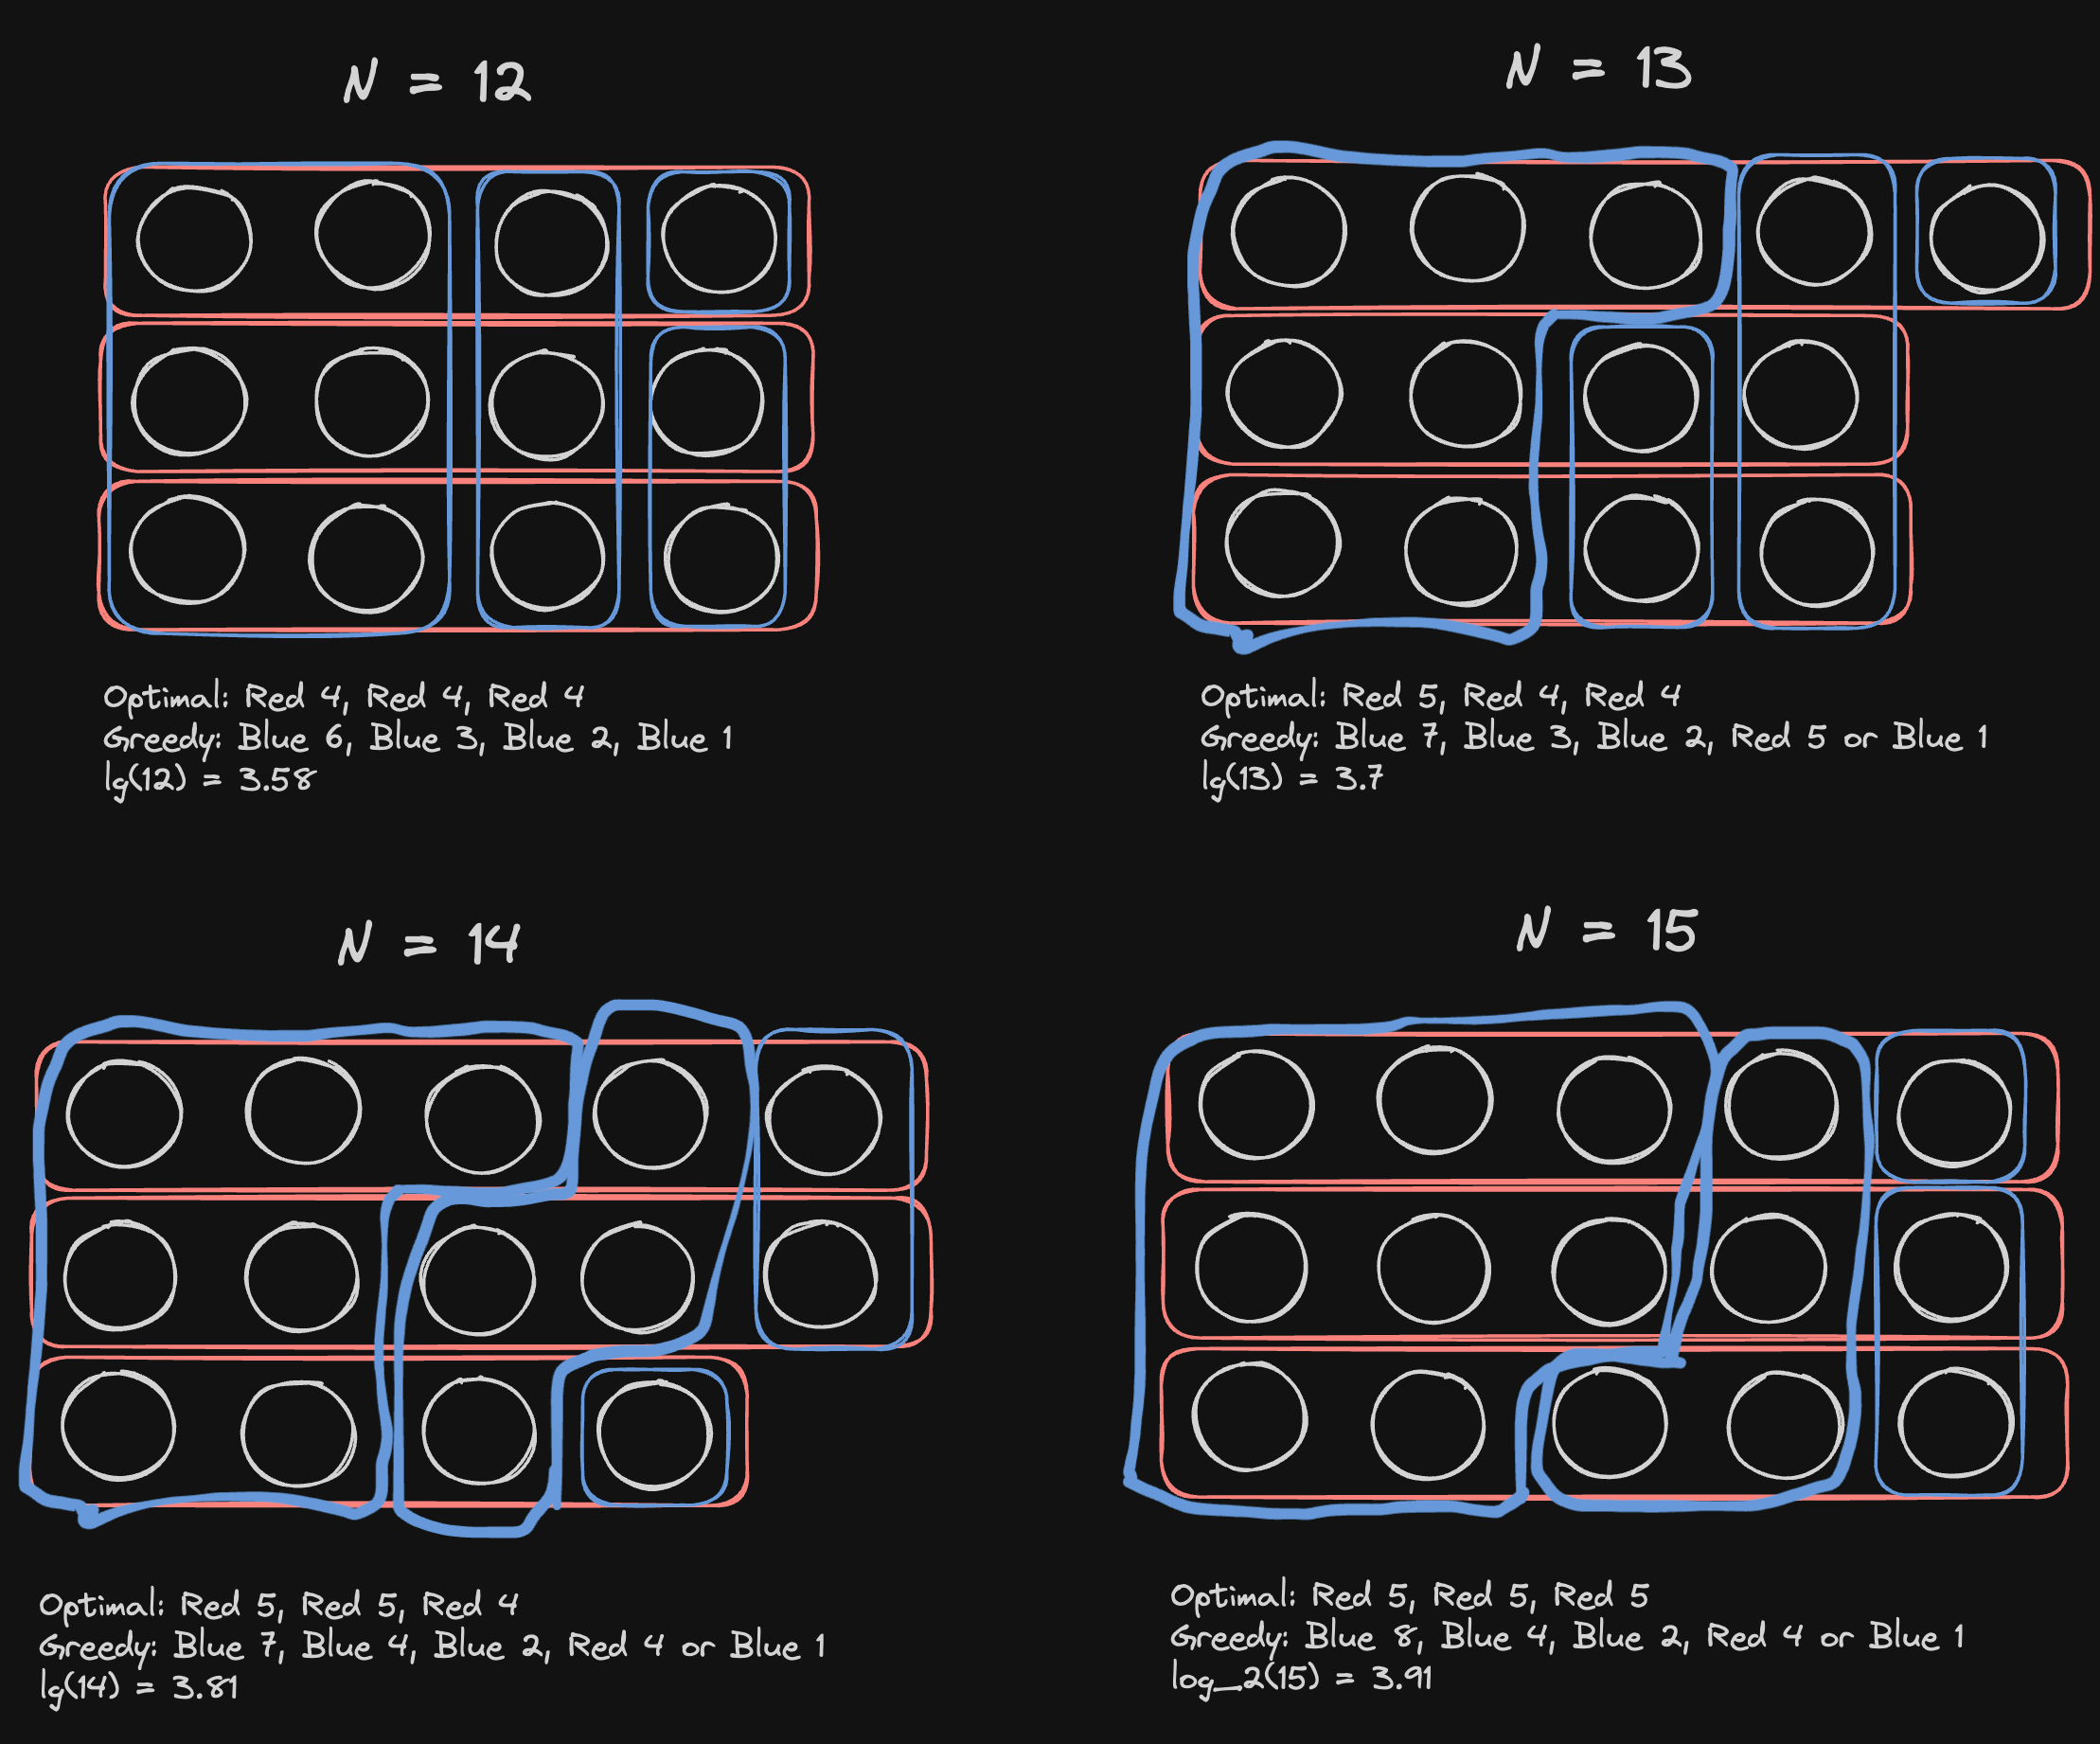
\includegraphics[scale=0.45]{./pics/q4_sets.png}
\medskip
\end{quote}


\item {\bf Tracking components in an evolving graph (15 points)}
% ``Hey Upper East Siders, Gossip Girl here." 
You are secretly Gossip Girl, an anonymous gossip blogger who keeps track of friendships at Constance Billard High School. You publish an up-to-date map of the friendships at Constance on your website.\footnote{There are no ethical concerns here, because you're a character in a highly-rated teen drama.} You maintain this map by a stream of distinct tips from anonymous followers of the form ``A is now friends with B." 

\begin{enumerate}
\item {\bf (5 points)}
    You call some groups of people a ``squad'': each person is in the same squad as all their friends, and every member of a squad has some chain of friendships to every other member. For example, if Dan is friends with Serena, Serena is friends with Blair, and Alice is friends with Donald, then Dan, Serena, and Blair are a squad (You make up the name ``The Gossip Girl Fan Club'') and Alice and Donald are another squad (``The Constance Constants''). Give an algorithm that takes in a stream of (a) tips and (b) requests for a specified person's squad name. You should answer requests that come in between tips consistently---if you make up the name ``The Billard billiards players'' for Dan's squad, and you're asked for Serena's squad's name before any new tips come in, you should report that it's ``The Billard billiards players''.
\item {\bf (10 points)}
    A ``circular squad'' is defined to be a squad such that there is some pair of friends within the group that have both a friendship and a chain of friendships of length more than 1. In the example above, if Dan and Blair also became friends, then the group would be a circular squad. If Dan and Donald also became friends, they would all be in one circular squad. Modify your algorithm from the previous part so that you report names that contain the word ``circle'' for all circular squads (and not for any other squads).
\end{enumerate}

\item {\bf Greedy scheduling (35 points)} Consider the following scheduling problem: we have two machines,
and a set of jobs $j_1,j_2,j_3,\ldots,j_n$ that we have to process.
To process a job, we need to assign it to one of the two machines;
each machine can only process one job at a time. 
Each job $j_i$ has an associated positive integer running time $r_i$.  The load on the 
machine is the sum of the running times of the jobs assigned to  it. 
The goal is to minimize the completion time, which is the maximum of the load of the two machines.  

Suppose we adopt a greedy algorithm: for every $i$, job $j_i$ is assigned to the
machine with the minimum load after the first $i-1$ jobs.  (Ties can
be broken arbitrarily.) 
\begin{enumerate}
\item
{\bf (5 points)} 
For all $n > 3$, give an instance of this problem for which
the completion time of the assignment of the greedy algorithm is a factor of $3/2$ away from the best
possible assignment of jobs.
\item
{\bf (15 points)}
Prove that the greedy algorithm always yields a completion
time within a factor of 3/2 of the best possible placement of jobs.
(Hint: Think of the best possible placement of jobs.  Even for the
best placement, the completion time is at least as big as the biggest
job, and at least as big as half the sum of the jobs.  You may want to
use both of these facts.)
\item
{\bf (10 points)} 
Suppose now instead of 2 machines we have $m$ machines and the completion time is defined as the maximum load over all the $m$ machines.  
Prove the best upper bound you can on the ratio of the 
performance of the greedy solution to the optimal solution, as a
function of $m$? 
\item
{\bf (5 points)} 
Give a family of examples (that is, one for
each $m$ -- if they are very similar, it will be easier to write
down!) where the factor separating the optimal and the greedy solutions
is as large as you can make it.
\end{enumerate}


\end{enumerate}

\end{document}
